\chapter{Putting a Price Tag on Life}

This chapter follows Michael Sandel's second lecture in Justice, presented here in companion-note form for the LazyLearn track and curated by LazyingArt LLC. We return from Dudley and Stephens to Bentham because Sandel wants to do more than revisit a dramatic case. He wants to know whether the impulse to count lives, pains, and benefits can be turned into a general moral principle. The lecture therefore begins with a clean rule, pushes that rule into public policy, and then tests whether the rule survives its own consequences.

\section{Returning to Bentham from the Lifeboat Case}

Sandel opens with a recap: last time we argued about the lifeboat case, the case of cannibalism at sea, and now we turn back to Bentham. The order matters. Utilitarianism is not introduced as an abstract doctrine dropped from the sky. It is introduced as a way of making systematic the sort of reasoning to which the lifeboat case had already tempted us.

Sandel's brief sketch of Bentham's life serves a purpose. Bentham goes to Oxford at twelve, to London at fifteen, to law at sixteen, and then gives his life not to legal practice but to jurisprudence and moral philosophy. The biographical sketch is there to mark the ambition of the doctrine: this is meant to be a general principle of morals and politics.

\begin{definition}
Bentham's principle of utility says that the highest principle of morality, whether personal or political, is to maximize the general welfare, or the collective happiness, or the balance of pleasure over pain.
\end{definition}

Sandel states the principle in prose. For compactness we may write
\begin{equation}
U = H - S,
\end{equation}
where \(H\) denotes happiness or pleasure and \(S\) denotes suffering or pain. This notation is editorial shorthand, but it tracks the lecture closely.

Bentham's next move is to extend the same logic from one person to the community. A community, he says, is the sum of the individuals who comprise it. If we compress that idea into a single formula, we obtain
\begin{equation}
U_{\text{community}}=\sum_{i=1}^{N} u_i.
\end{equation}
Once the problem is written in this way, the political rule becomes immediate:
\begin{equation}
a^\star=\arg\max_a U(a).
\end{equation}
The right act, the right policy, and the right law are the ones that maximize utility.

This is the first mathematical spine of the lecture. It is elementary in form, but it is powerful in implication. If we can identify the relevant benefits and costs, and if those benefits and costs can be placed on a common scale, then legislation begins to look like a problem of comparison and optimization.

\section{Cost-Benefit Analysis as Utilitarianism in Practice}

Sandel's first major pivot is from principle to mechanism. Utilitarianism, he says, often appears in contemporary life under the name of cost-benefit analysis. The language changes, but the form does not. We list the benefits, list the costs, and compare the totals.

For a policy \(a\), the operational rule is
\begin{equation}
\text{Net}(a)=\text{Benefits}(a)-\text{Costs}(a).
\end{equation}
At this stage the logic seems almost irresistible. What could be more reasonable than counting up the benefits of a policy and subtracting its burdens?

The Czech smoking case is Sandel's first stress test. Philip Morris commissioned a cost-benefit study of smoking in the Czech Republic, and the study concluded that the government gains by having citizens smoke. Sandel then walks us through the ledger. On one side lie the negative effects: increased health-care costs for smoking-related disease. On the other side lie tax revenues, pension savings, savings in health care when people die earlier, and even savings in housing costs for the elderly. In a compact ledger form,
\begin{align}
\text{Net}_{\text{Czech smoking}}
&=\text{tax revenue}
+\text{health-care savings from early death} \nonumber\\
&\quad+\text{pension savings}
+\text{housing savings}
-\text{smoking-related health costs} \nonumber\\
&=\$147\,\text{million}.
\end{align}
At the individual level, the same reasoning yields
\begin{equation}
\text{savings per premature death} > \$1200.
\end{equation}

The arithmetic is not presented as a parody. Sandel lets it run in its own terms. That is what gives the example its force. Early death now enters the calculation as a fiscal gain. The lecture's moral pressure does not come from any algebraic mistake. It comes from the spectacle of a coherent ledger whose coherence seems itself offensive.

At once Sandel anticipates the utilitarian reply. Perhaps this is an unfair test. Philip Morris was pilloried in the press and apologized. A defender of utilitarianism may say that the calculation omitted what matters most: the value of the life lost, the loss to the person, and the loss to the family. If those terms were added to the ledger, perhaps the result would reverse. Sandel accepts that this is the natural reply, and then moves to a case designed precisely to test it.

\section{Ford Pinto, Cell Phones, and the Price of Life}

The Ford Pinto case is Sandel's harder test. Here, unlike in the Czech example, the company does assign a dollar value to life and injury. So the question becomes sharper: if the life term is entered explicitly, does that save cost-benefit reasoning, or does it expose its problem more clearly?

Ford knew that the Pinto's rear fuel tank was vulnerable in collisions and considered adding a protective shield. The safety improvement was estimated at \(\$11\) per car across \(12.5\) million cars and trucks:
\begin{equation}
C_{\text{Pinto safety}}=(\$11)\cdot(12.5\times 10^6)\approx \$137\,\text{million}.
\end{equation}
The transcript's arithmetic is approximate here, as Sandel reports \(\$137\) million rather than \(\$137.5\) million, but the structure is clear.

The benefit side of the memo included expected deaths, expected injuries, and the value of vehicles that would otherwise be destroyed. Because the injury coefficient is garbled in the transcript, it is safest to keep that term symbolic:
\begin{equation}
B_{\text{Pinto safety}}
=
180(\$200{,}000)+180I+2000(\$700)\approx \$49.5\,\text{million},
\end{equation}
where \(I\) denotes the memo's injury valuation. The decision then follows from the sign of the difference:
\begin{align}
\Delta_{\text{Pinto}}
&=B_{\text{Pinto safety}}-C_{\text{Pinto safety}} \nonumber\\
&\approx \$49.5\,\text{million}-\$137\,\text{million} \nonumber\\
&\approx -\$87.5\,\text{million}.
\end{align}
So the device is not installed.

This is one of the lecture's strongest numerical examples because the arithmetic is so plain. If benefits are lower than costs, the improvement is rejected. What horrifies the jurors is not that the memo forgot to count life. It counted life explicitly.

Sandel then widens the frame. The same form appears in policy debates over cell-phone use while driving. A study is said to find roughly \(2000\) annual deaths from such use; later, in the live exchange, Sandel rounds the figure up to \(2300\). Against these deaths are placed the economic and practical gains from using travel time for business, coordination, and ordinary convenience. The resulting structure is again the same:
\begin{equation}
\text{Net}_{\text{cell phone}}
\approx
\text{convenience and economic benefit}
-
N_{\text{deaths}}V_{\text{life}}.
\end{equation}
The point is not that the lecture settles the cell-phone question. The point is that once \(V_{\text{life}}\) is introduced, the issue appears to fit the same calculus as the Pinto memo.

\subsection{Question \& Answer}

\paragraph{}
Can human life be given a dollar value without distorting the moral problem?

\paragraph{}
Sandel's classroom exchange produces two answers. One answer says that the problem is numerical. If Ford valued a death at \(\$200{,}000\), then the figure was far too low. On this view the calculus itself is sound; it merely needs a more realistic price, whether \(\$1\) million, \(\$2\) million, or some other figure.

\paragraph{}
The other answer says that the problem lies deeper. Julia's response captures it sharply: the mistake is not that the number is too low, but that human life should not be handled by this monetary device at all. What is lost is not only money or earnings, but a person and a set of human relationships, and those losses may be misdescribed the moment they are entered as a price.

\paragraph{}
The lecture does not yet decide between these two replies. What it does is more important structurally. It forces the issue from a technical dispute about inputs to a philosophical dispute about the form of the calculation itself. That shift opens the way to Sandel's two objections to Bentham.

\section{Two Objections to Bentham: Rights and Commensurability}

Sandel now steps back from the cases and asks what, exactly, the objections are. He does not want the lecture to remain a collection of appalled reactions. He wants the pressure points named cleanly.

The first objection concerns rights, especially the rights of minorities and individuals. Anna voices this worry in the classroom: the fact that a person belongs to the smaller number does not mean that his claims matter less. Youngda replies in a perfectly Benthamite way that each person's preference still counts; the difficulty is that the larger number outweighs the smaller. Sandel then presses the point with examples. The boy in the lifeboat had as much right to live as the others. A suspected terrorist may possess rights even if torturing him might save thousands. And the Roman arena case states the difficulty in the starkest way: a few victims suffer horribly, a crowd exults, and pure aggregation threatens to justify the spectacle if the crowd is large enough.

The second objection concerns commensurability. Even if we agreed to aggregate, can all goods, losses, and human concerns be translated into a single scale? Thorndike's survey is introduced as an attempt to show that they can. Respondents assigned dollar amounts to unlike experiences: pulling a tooth, cutting off a toe, eating a worm, living the rest of one's life on a farm in Kansas, choking a stray cat. The resulting ranking is exactly the kind of thing Sandel wants us to inspect:
\begin{equation}
V(\text{Kansas})=\$300{,}000
>
V(\text{eat earthworm})=\$100{,}000
>
V(\text{pull tooth})=\$4{,}500.
\end{equation}
The ranking is not interesting because it is silly. It is interesting because the silliness may reveal something true: perhaps these goods and harms are being misshapen by the very act of being forced into one scale.

Sandel's St.\ Anne's story makes the same point with more social texture. Traditional objections to overnight male guests at a women's college were translated into utilitarian housekeeping costs: baths, hot water, mattresses, and finally a fee of \(50\) pence per night. The headline that followed showed at once how translation into a cost schedule can destroy the meaning of what is being discussed. A question of moral convention had become a price tag.

At this point Sandel explicitly consolidates the argument. We are looking at two different objections: one about whether utilitarianism respects rights, and the other about whether all values are commensurable at all.

\begin{figure}
\centering
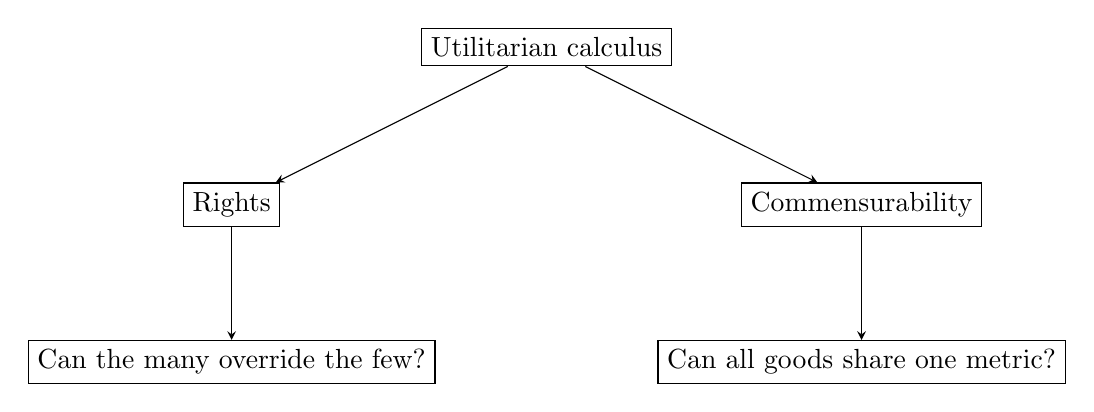
\begin{tikzpicture}[>=stealth]
\node[draw, rectangle] (u) at (0,2) {Utilitarian calculus};
\node[draw, rectangle] (r) at (-4,0) {Rights};
\node[draw, rectangle] (c) at (4,0) {Commensurability};
\node[draw, rectangle] (rr) at (-4,-2) {Can the many override the few?};
\node[draw, rectangle] (cc) at (4,-2) {Can all goods share one metric?};
\draw[->] (u) -- (r);
\draw[->] (u) -- (c);
\draw[->] (r) -- (rr);
\draw[->] (c) -- (cc);
\end{tikzpicture}
\end{figure}

The diagram is only a map, but it captures an important pedagogical beat. The lecture has moved from examples to a formal branching of the problem.

\section{Bentham on Quantity, Not Quality}

Sandel's next pivot is subtle. Up to now we have asked whether we may add all goods together. He now asks a different question: even if we could add them, why should we count every preference without asking whether it is a good preference or a bad one?

Bentham's answer is that we should refuse such qualitative rankings. What matters are the intensity and duration of pleasure and pain. The slogan Sandel gives is the famous one: the quantity of pleasure being equal, pushpin is as good as poetry. In a deliberately schematic shorthand, we may write
\begin{equation}
\operatorname{Qty}(p_1)=\operatorname{Qty}(p_2)\Longrightarrow p_1\sim p_2.
\end{equation}
The notation is only a compression of Bentham's claim. If the quantity is the same, the ranking is the same.

Sandel is careful to show why this view is attractive. It looks egalitarian. It refuses to let one class of people declare another class's pleasures intrinsically inferior. Mozart versus Madonna, ballet versus bowling: who is to judge? Bentham's refusal to judge carries a democratic appeal.

But the lecture now has enough material on the table to challenge that flatness. The Roman crowd's delight in blood sport does not look like just another pleasure of equal standing. Here the objection is not only that Christians are wronged. It is also that the crowd's pleasure seems base and degrading. So the question becomes unavoidable: can a utilitarian distinguish higher from lower pleasures without abandoning utilitarianism? That question is the bridge to Mill.

\section{Mill's Repair: Higher Pleasures and the Competent Judge}

Mill enters, in Sandel's presentation, as a reformer from within. The brief biography is not ornamental. It marks Mill's inheritance and his burden. James Mill, Bentham's disciple, gives his son an extreme education: Greek at three, Latin at eight, Roman law at ten. Then comes the breakdown, the depression, and eventually Harriet Taylor, under whose influence Mill tries to humanize utilitarianism.

Mill's first move is not to reject utility. On the contrary, he affirms it emphatically. The desirable, he says, is what people do in fact desire. So the repair must work from within the field of actual preference, not by appealing to a mysterious moral faculty outside it.

\begin{definition}
Mill's competent-judge test says that of two pleasures, the higher pleasure is the one that all or almost all who have experienced both decidedly prefer, and prefer independently of any external feeling of moral obligation.
\end{definition}

A compact way to summarize the structure is
\begin{equation}
\text{Higher}(p_1,p_2)
\iff
\text{those acquainted with both }p_1\text{ and }p_2\text{ decidedly prefer }p_1.
\end{equation}
The significance of the definition lies in what it excludes. Mill does not permit us to step outside actual preference. He does, however, restrict the relevant preferences to those of people who know both sides of the comparison.

\subsection{Question \& Answer}

\paragraph{}
How can a utilitarian distinguish higher from lower pleasures without leaving utilitarian premises?

\paragraph{}
Mill's answer is that we do not leave the premises at all. We remain with desire and preference. But we do not consult just any desire. We ask those who have experienced both alternatives which one they decidedly prefer.

\paragraph{}
This is why Mill can say that some pleasures are higher without appealing to an independent moral yardstick. The higher pleasure is not the one pronounced noble by some external authority. It is the one preferred by those competent to compare.

\paragraph{}
The repair is ingenious, but it is also delicate. The class of competent judges is typically educated, cultivated, and able to appreciate what crude preference might miss. So the distinction between recording preferences and educating preferences begins to narrow. Sandel does not suppress this tension. He prepares to test it in public.

\section{Shakespeare, The Simpsons, Rights, and the Limits of the Repair}

Sandel's test is the classroom experiment with Hamlet, Fear Factor, and The Simpsons. Its force depends on the two-stage structure. First the room is asked what it likes most. Then it is asked what it regards as the higher or worthier experience. If those two questions yield different answers, Mill has gained an important foothold.

\begin{table}
\centering
\begin{tabular}{lll}
Question posed & Dominant response & Philosophical use \\
Most liked & The Simpsons & immediate preference \\
Highest experience & Shakespeare & qualitative ranking \\
\end{tabular}
\end{table}

This is the live form of Mill's claim:
\begin{equation}
\text{Preferred} \neq \text{Higher}.
\end{equation}
The room's immediate taste and its reflective ranking do not coincide. That gap is exactly what Bentham's flat metric has trouble recognizing.

The subsequent discussion deepens the point. One student suggests that Shakespeare seems higher only because culture teaches us to say so. Another replies that if one had to live for the rest of one's life with one body of material, the richer work would sustain a deeper mental life. Joe's answer is especially important for the lecture's rhythm: what we like in the moment is not necessarily what we would choose for a life.

The rat example pushes the same contrast into a simpler biological frame. A rat can stimulate its own brain and experience intense pleasure to the point of death. That shows intensity; it does not show the superiority of the life. Mill's point is that human beings who know both sides of the comparison would prefer a life of higher faculties, even if it includes dissatisfaction.

At this point Sandel broadens the repair from pleasures to rights. Mill's claim is that justice is not a foreign body within utilitarianism. It is the chief and most sacred part of morality because, regarded collectively, it stands higher in the scale of social utility. If we want a symbolic shorthand for the order Mill is trying to assert, we may write
\begin{equation}
\text{Justice and rights} \succ \text{other moral requirements}.
\end{equation}
The relation is ordinal, not numerical. Mill is not giving us a meter for justice. He is claiming that, once long-run human interests are considered, rights deserve a privileged place within the utilitarian scheme.

This is where the lecture deliberately stops short of closure. Has Mill repaired utilitarianism, or has he smuggled in non-utilitarian standards while still using the vocabulary of utility? Sandel refuses to settle the matter prematurely. The unresolved question is part of the intellectual work of the lecture.

The Bentham coda then returns us to the founder. Bentham's preserved body, his wax head, his insistence that even a dead philosopher should be useful: these details are funny, but not merely funny. They show a thinker who remained faithful to his principle in life and in death. The story closes the lecture in the right way. Bentham is not dismissed. He is left before us as both rigorous and unsettling.

\section{Summary}

We began with Bentham's simple rule that the right act or policy maximizes utility. We then watched that rule become operational in cost-benefit analysis, where benefits are added, costs are subtracted, and decisions follow from the sign of the result. The Czech smoking study and the Ford Pinto memo showed how far that arithmetic can reach once life itself receives a monetary term.

From there the lecture extracted two objections. The first was about rights: perhaps the good of the many cannot justify the sacrifice of the few. The second was about commensurability: perhaps not all goods and harms belong on one common scale in the first place. Bentham's own answer was to count quantity rather than quality. Mill's answer was to preserve utility while distinguishing higher pleasures and giving justice a privileged place in the long run. Whether that answer truly remains inside utilitarianism is the question Sandel leaves suspended, and it is the right question with which to end.